
% Copyright (c) 2015 - 2020 Mario Mlačak, mmlacak@gmail.com
% Licensed and published as Public Domain work.

% Hemera's Dawn chapter ===============================================
\chapter*{Hemera's Dawn}
\addcontentsline{toc}{chapter}{Hemera's Dawn}
\label{ch:Hemera's Dawn}

\begin{flushright}
\parbox{0.8\textwidth}{
\emph{Then assuredly the world was made, not in time, but simultaneously with time. \\
\hspace*{\fill}{\textperiodcentered \textperiodcentered \textperiodcentered \hspace*{0.2em} St. Augustine} } }
\end{flushright}

\noindent
Hemera's Dawn is chess variant which is played on 20 x 20 board, with
darkish red-brown and grey fields and pure red and bright yellow pieces.
Star colors are bright blue and white. In algebraic notation, columns
are enumerated from 'a' to 't', and rows are enumerated from '1' to '20'.
Three new pieces are introduced; Centaur, Scout, and Grenadier; with
algebraic symbols 'C', 'O', and 'G', respectively.

\clearpage % ..........................................................
% Centaur *************************************************************

\section*{Centaur}
\addcontentsline{toc}{section}{Centaur}
\label{sec:Hemera's Dawn/Centaur}

\noindent
\begin{wrapfigure}[12]{l}{0.4\textwidth}
\centering
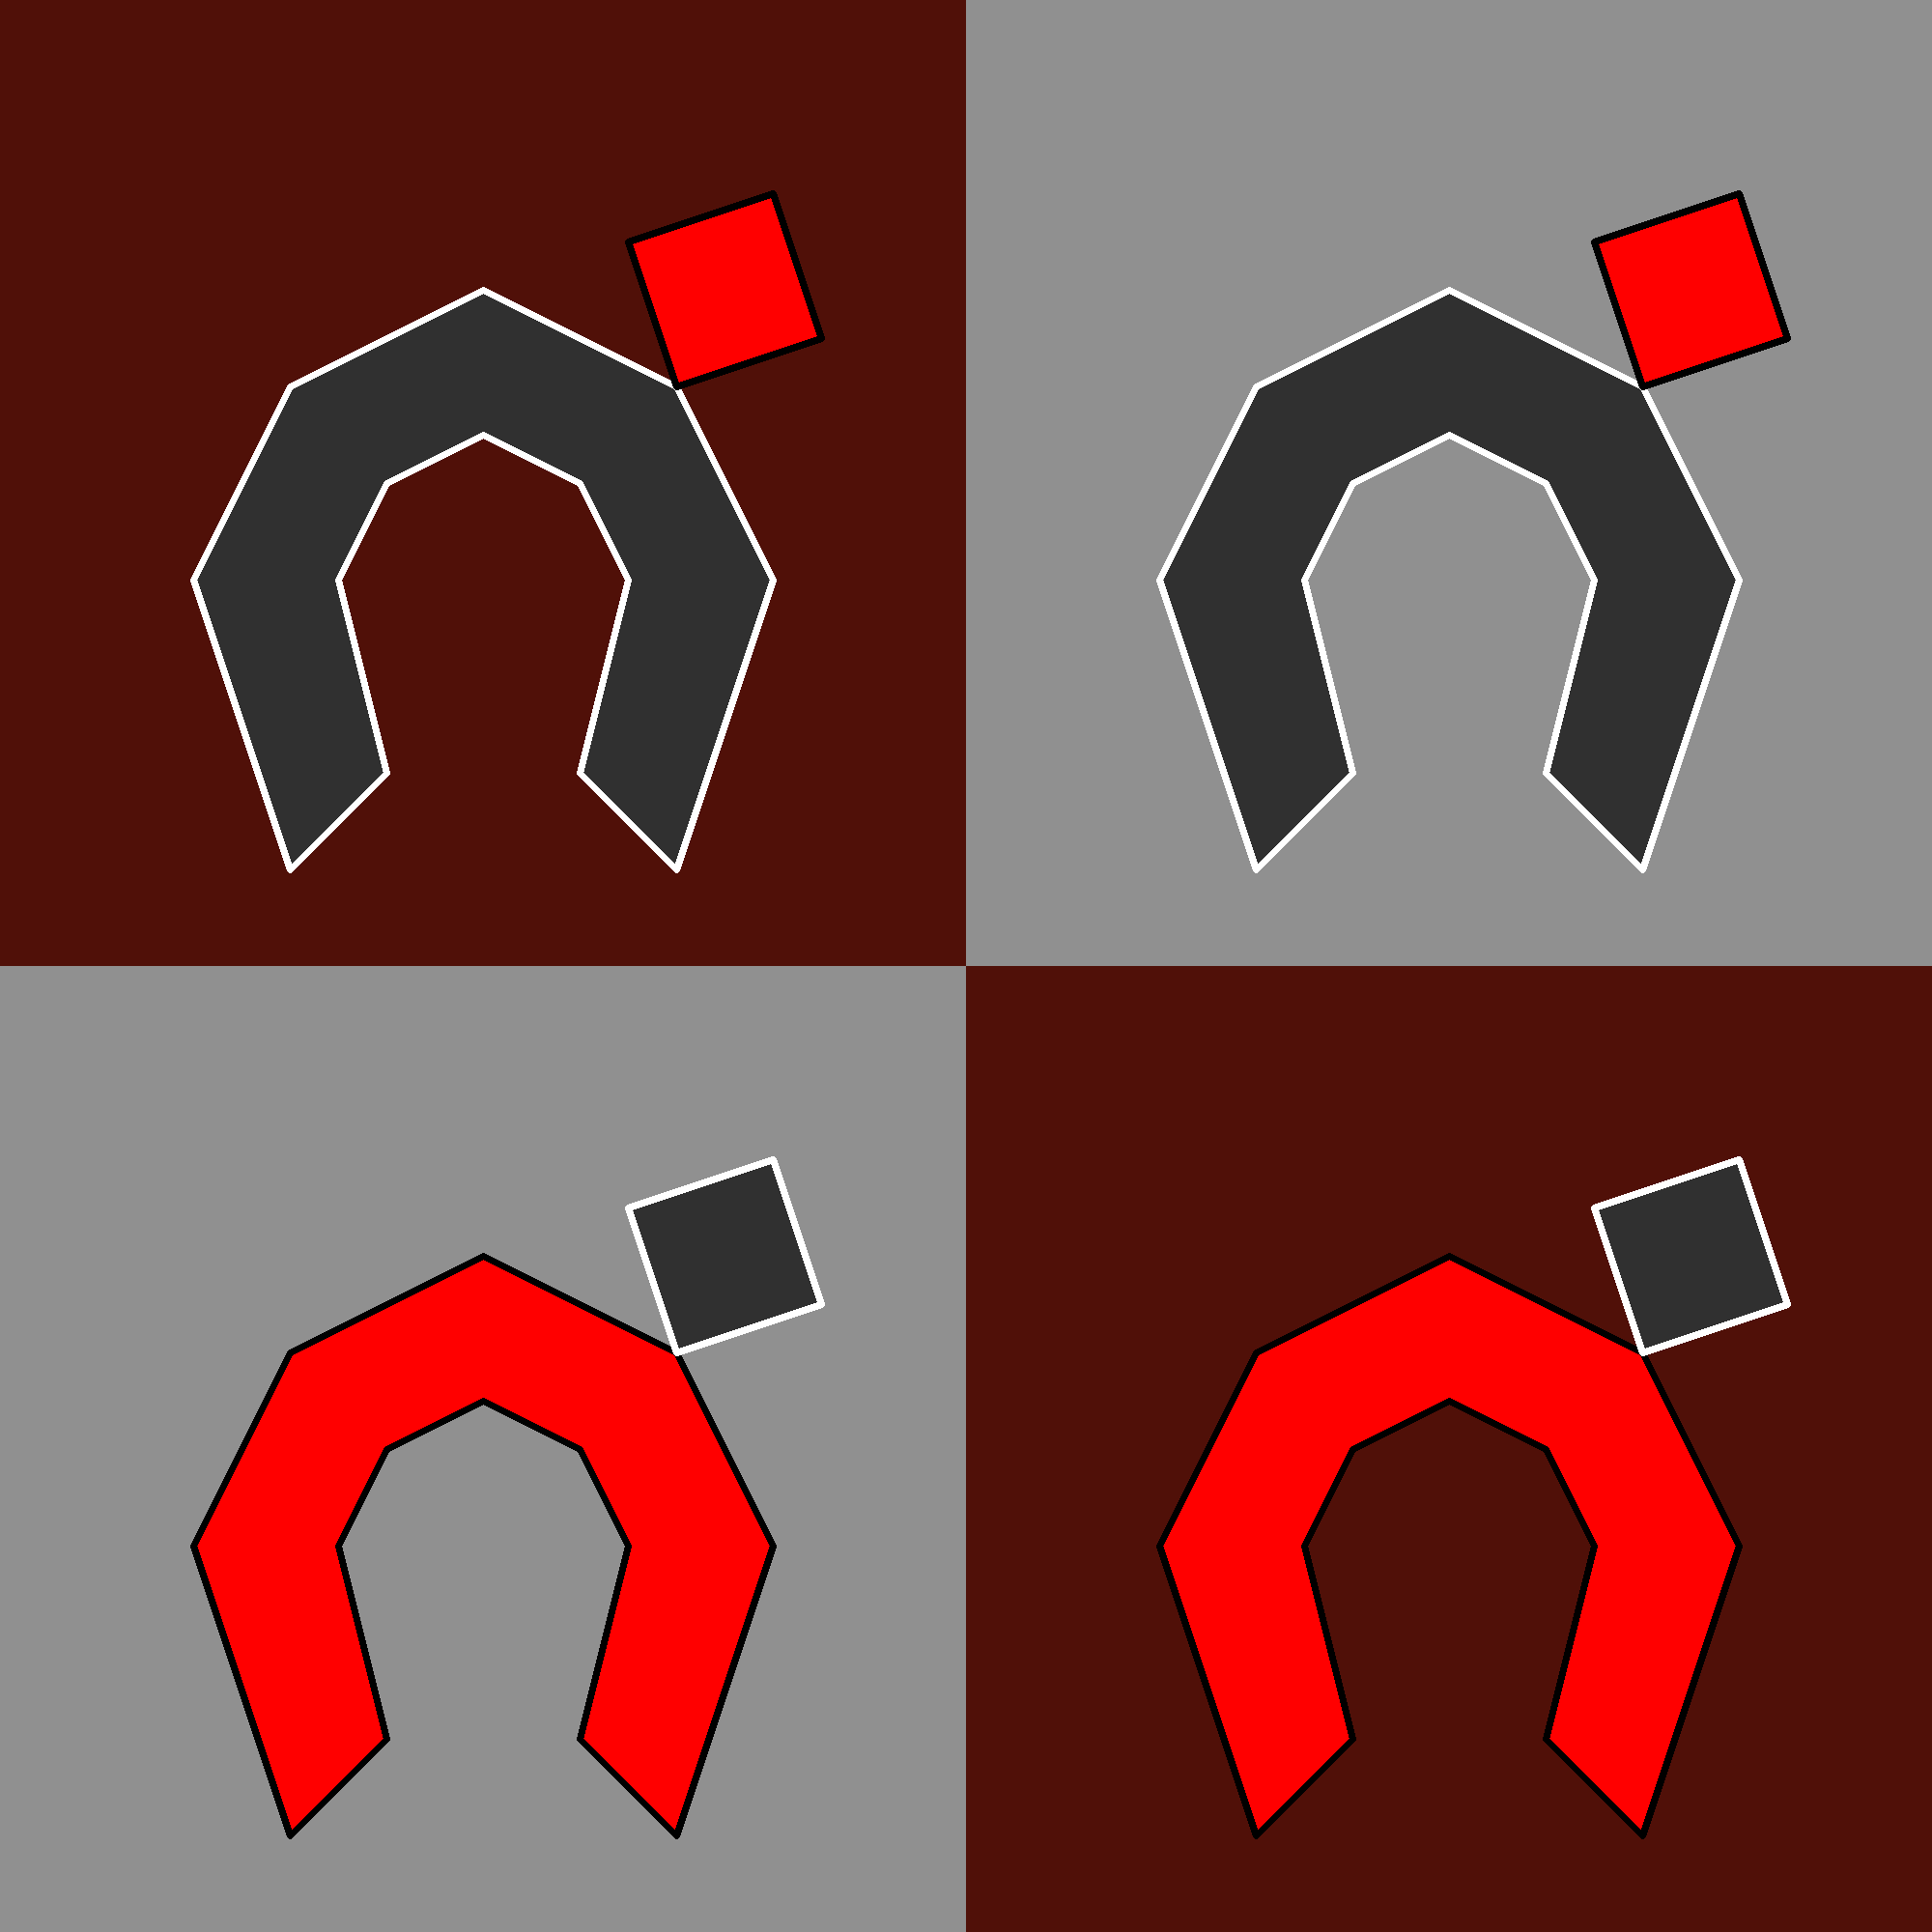
\includegraphics[width=0.4\textwidth, keepaspectratio=true]{pieces/12_centaur.png}
\caption{Centaur}
\label{fig:12_centaur}
\end{wrapfigure}
Centaur is similar to Unicorn, only it can continue its jumpy movement
in two chosen directions until another piece is encountered, or it runs
out of a chessboard.

First direction is chosen freely, second direction is limited by the first
choice. Once both long and short jump directions are determined, Centaur
has to follow them in all subsequent steps, for the remainder of that ply.

For Centaur's ply to be legal, all steps must end up on the chessboard.
Unlike Wave, Centaur cannot step outside of a chessboard, and in later
step(s) return back onto it.

\noindent
\begin{wrapfigure}{l}{0.4\textwidth}
\centering
\includegraphics[width=0.4\textwidth, keepaspectratio=true]{pieces/star/14_hemera_s_dawn.png}
\caption{Star}
\label{fig:star/14_hemera_s_dawn}
\end{wrapfigure}
Star colors in this variant are different to colors of light and dark pieces.

\clearpage % ..........................................................
% Movement ------------------------------------------------------------

% \vspace{7\baselineskip}
\subsection*{Movement}
\addcontentsline{toc}{subsection}{Movement}
\label{sec:Hemera's Dawn/Centaur/Movement}

% \vspace*{-1.1\baselineskip}
\vspace*{-0.7\baselineskip}
\noindent
\begin{minipage}{\textwidth}
\begin{wrapfigure}[9]{l}{0.4\textwidth}
\centering
\includegraphics[width=0.35\textwidth, keepaspectratio=true]{examples/14_hd/scn_hd_01_centaur_same_color.png}
\vspace*{-0.7\baselineskip}
\caption{Centaur short jump}
\label{fig:scn_hd_01_centaur_same_color}
\end{wrapfigure}
On fields with the same color as Centaur, it has the same step-fields (green, blue)
as Knight has.

\mbox{}\newline % Forcing new paragraph ...
On fields in opposite color, Centaur can jump much longer, and has the same step-fields
(green, blue) as Unicorn has. For comparison, short steps are also numbered (grey).
\end{minipage}

\vspace*{0.9\baselineskip}
\noindent
\begin{minipage}{\textwidth}
\begin{wrapfigure}[14]{l}{0.6\textwidth}
\centering
\includegraphics[width=0.55\textwidth, keepaspectratio=true]{examples/14_hd/scn_hd_02_centaur_opposite_color.png}
\vspace*{-0.7\baselineskip}
\caption{Centaur long jump}
\label{fig:scn_hd_02_centaur_opposite_color}
\end{wrapfigure}
Again, just as Knight (and Unicorn), Centaur is not hampered by a piece on any
unmarked field.

\mbox{}\newline % Forcing new paragraph ...
Step-fields are also capture-fields, Centaur would be able to capture opponent's
pieces on any marked field, regardless of marker color (green, blue).
\end{minipage}

\vspace*{0.7\baselineskip}
On initial step, Centaur can freely choose any marked field, regardless of marker
color (green, blue), or step (long, short). On second step, Centaur can choose any
step-field in the other color (blue if green was chosen initially, green if blue
was first choice). On all subsequent steps, Centaur has to keep alternating between
the two initially chosen steps, for the remainder of a ply.

\clearpage % ..........................................................

\noindent
\begin{figure}[!h]
\includegraphics[width=1.0\textwidth, keepaspectratio=true]{examples/14_hd/scn_hd_03_centaur_multi_step_init.png}
\caption{Centaur initial step}
\label{fig:scn_hd_03_centaur_multi_step_init}
\end{figure}

Here, light Centaur is located on the same color (i.e. light) field, so all available
step-fields are short jumps, which are the same as those of Knight. For the first step,
Centaur can choose any of marked step-fields, except the one which is blocked by own
piece (light Pawn).

\clearpage % ..........................................................

\noindent
\begin{figure}[!h]
\includegraphics[width=1.0\textwidth, keepaspectratio=true]{examples/14_hd/scn_hd_04_centaur_multi_step_second.png}
\caption{Centaur second step}
\label{fig:scn_hd_04_centaur_multi_step_second}
\end{figure}

Here, after first step, light Centaur is located on a dark field, so all available
step-fields are long jumps, which are the same as those of Unicorn. Since upper-left
step-field (blue) was chosen for a first step, next step has to be one of upper-right,
lower-left fields (green). Note, opponent's piece (dark Pawn) can be captured, but it
blocks light Centaur from moving any further.

\clearpage % ..........................................................

\noindent
\begin{figure}[!h]
\includegraphics[width=1.0\textwidth, keepaspectratio=true]{examples/14_hd/scn_hd_05_centaur_multi_step.png}
\caption{Centaur complete move}
\label{fig:scn_hd_05_centaur_multi_step}
\end{figure}

After second step is chosen, complete movement of Centaur consists of alternating
between the two initial steps. Centaur for the rest of a ply has to follow those two
initial steps, e.g. after reaching field 4, it cannot move to any other step-field
(red). Light Centaur could also capture dark Bishop, but is prevented from moving
any further (grey). Pieces on all other fields are ignored (Pawns).

\clearpage % ..........................................................

\subsubsection*{Out of board steps}
\addcontentsline{toc}{subsubsection}{Out of board steps}
\label{sec:Hemera's Dawn/Centaur/Movement/Out of board steps}

% \vspace*{-0.05\textwidth}
\vspace*{-1.3\baselineskip}
\noindent
\begin{figure}[!h]
\includegraphics[width=1.0\textwidth, keepaspectratio=true]{examples/14_hd/scn_hd_06_centaur_off_board.png}
\caption{Centaur off-board steps}
\label{fig:scn_hd_06_centaur_off_board}
\end{figure}

Here, light grey fields are virtual fields extending existing chessboard. For
Centaur, it's illegal to step outside of a chessboard, and all subsequent steps
are also illegal.

Here, Centaur cannot reach fields 1 and 2 from starting position with selected
directions, even though it would end movement on the chessboard.

% ------------------------------------------------------------ Movement
\clearpage % ..........................................................
% Activating Wave -----------------------------------------------------

\subsection*{Activating Wave}
\addcontentsline{toc}{subsection}{Activating Wave}
\label{sec:Hemera's Dawn/Centaur/Activating Wave}

\vspace*{-1.3\baselineskip}
\noindent
\begin{figure}[!h]
\includegraphics[width=1.0\textwidth, keepaspectratio=true]{examples/14_hd/scn_hd_07_wave_activation_by_centaur_first_step.png}
\caption{Wave activation by Centaur, first step}
\label{fig:scn_hd_07_wave_activation_by_centaur_first_step}
\end{figure}

Wave activated by Centaur, \hyperref[fig:scn_hd_01_centaur_same_color]{moves like one}.
Here, light Wave is activated on the opposite color (i.e. dark) field, so all available
step-fields are long jumps, which are the same as those of Unicorn. For the first step,
Wave can choose any of marked step-fields (green, blue), including the one occupied by
own piece (light Pawn). Light Pawn could be activated, or stepped over.

\clearpage % ..........................................................

% \vspace*{-1.0\baselineskip}
\noindent
\begin{figure}[!h]
\includegraphics[width=1.0\textwidth, keepaspectratio=true]{examples/14_hd/scn_hd_08_wave_activation_by_centaur_second_step.png}
\caption{Wave activation by Centaur, second step}
\label{fig:scn_hd_08_wave_activation_by_centaur_second_step}
\end{figure}

After first step, light Wave is located on a light field, so all available step-fields
are short jumps, which are the same as those of Knight. Since upper-right step-field
(green) was chosen for a first step, next step has to be one of upper-left, lower-right
fields (blue). Light Wave cannot activate opponent's piece (dark Pawn), but it can step
over it.

\clearpage % ..........................................................

% \vspace*{-1.0\baselineskip}
\noindent
\begin{figure}[!h]
\includegraphics[width=1.0\textwidth, keepaspectratio=true]{examples/14_hd/scn_hd_09_wave_activation_by_centaur_complete.png}
\caption{Wave activation by Centaur}
\label{fig:scn_hd_09_wave_activation_by_centaur_complete}
\end{figure}

After second step is chosen, complete movement of Wave consists of alternating between
the two initially chosen steps, which Wave for the rest of a ply has to follow, e.g.
after reaching field 4, it cannot move to any other step-field (red). Light Wave could
also activate dark Wave, or it could continue moving further. Pieces on all other fields
are ignored (Pawns).

\clearpage % ..........................................................

\subsubsection*{Out of board steps}
\addcontentsline{toc}{subsubsection}{Out of board steps}
\label{sec:Hemera's Dawn/Centaur/Activating Wave/Out of board steps}

\vspace*{-1.2\baselineskip}
\noindent
\begin{figure}[!h]
\includegraphics[width=1.0\textwidth, keepaspectratio=true]{examples/14_hd/scn_hd_10_wave_activated_by_centaur_off_board.png}
\caption{Wave off-board steps}
\label{fig:scn_hd_10_wave_activated_by_centaur_off_board}
\end{figure}

Again, light grey fields are virtual fields extending existing chessboard.
Wave activated by Centaur can step outside of a board, as long as its ply
ends on a board, just like
\hyperref[fig:scn_mv_25_wave_off_board]{Wave activated by Unicorn}. Here,
step-fields 1 and 2 are reachable by Wave, even though it stepped outside
of the board. It is illegal for any piece, including Wave, to end its ply
outside of a board.

\clearpage % ..........................................................

\subsection*{Teleporting Wave}
\addcontentsline{toc}{subsection}{Teleporting Wave}
\label{sec:Hemera's Dawn/Centaur/Teleporting Wave}

\vspace*{-1.2\baselineskip}
\noindent
\begin{figure}[!h]
\includegraphics[width=1.0\textwidth, keepaspectratio=true]{examples/14_hd/scn_hd_11_wave_teleport.png}
\caption{Wave off-board teleporting}
\label{fig:scn_hd_11_wave_teleport}
\end{figure}

Activation by Centaur and following teleportation of Wave is
\hyperref[fig:scn_n_07_teleport_wave_init]{exactly the same as if activated by Unicorn},
except Wave can now carry more than 1 momentum, because Centaur's ply can be
longer than just 1 step.

% ----------------------------------------------------- Activating Wave
% ************************************************************* Centaur
\clearpage % ..........................................................
% Scout ***************************************************************

\section*{Scout}
\addcontentsline{toc}{section}{Scout}
\label{sec:Hemera's Dawn/Scout}

\vspace*{-0.7\baselineskip}
\noindent
\begin{wrapfigure}[6]{l}{0.4\textwidth}
\centering
\includegraphics[width=0.4\textwidth, keepaspectratio=true]{pieces/13_scout.png}
\vspace*{-1.3\baselineskip}
\caption{Scout}
\label{fig:13_scout}
\end{wrapfigure}
Scout is more mobile relative of a Pawn. Like Pawn, Scout can rush, and can be captured
by en passant. Unlike Pawn, Scout cannot be promoted. Pawns can be pomoted to Scouts.

\vspace*{4.1\baselineskip}
\subsection*{Scout-fields}
\addcontentsline{toc}{subsection}{Scout-fields}
\label{sec:Hemera's Dawn/Scout/Scout-fields}

\vspace*{-0.7\baselineskip}
\noindent
\begin{wrapfigure}[5]{l}{0.4\textwidth}
\centering
\includegraphics[width=0.25\textwidth, keepaspectratio=true]{examples/14_hd/scn_hd_14_scout_fields.png}
\vspace*{-0.3\baselineskip}
\caption{Scout-fields}
\label{fig:scn_hd_14_scout_fields}
\end{wrapfigure}
Scout-fields are all fields immediately neighboring Scout horizontally,
vertically, and diagonally. They are the same fields as step-fields of a King.

% \clearpage % ..........................................................

\vspace*{1.1\baselineskip}
\subsection*{Movement}
\addcontentsline{toc}{subsection}{Movement}
\label{sec:Hemera's Dawn/Scout/Movement}

. . .

% \vspace*{7.3\baselineskip}
\TODO :: decide on Scout movement

\clearpage % ..........................................................

\subsection*{Rush}
\addcontentsline{toc}{subsection}{Rush}
\label{sec:Hemera's Dawn/Scout/Rush}

\TODO :: Rushing Scouts

\clearpage % ..........................................................

\subsection*{En passant}
\addcontentsline{toc}{subsection}{En passant}
\label{sec:Hemera's Dawn/Scout/En passant}

\TODO :: Capturing Pawns with Scouts using en passant

\clearpage % ..........................................................

\subsection*{Initial positions}
\addcontentsline{toc}{subsection}{Initial positions}
\label{sec:Hemera's Dawn/Scout/Initial positions}

\vspace*{-0.7\baselineskip}
\noindent
\begin{figure}[!h]
\includegraphics[width=1.0\textwidth, keepaspectratio=true]{examples/14_hd/scn_hd_16_scout_initial_positions.png}
\caption{Initial positions of Scouts}
\label{fig:scn_hd_16_scout_initial_positions}
\end{figure}

. . .

% In this variant an additional set of Pawns are added to
% \hyperref[fig:14_hemera_s_dawn]{the initial setup},
% called Scouts. Scouts do not make full-size Pawns ranks, and so their
% rows are not Pawns rows.

% Scouts are positioned relative to Centaurs' initial positions, to block them
% from capturing opponent's pieces from the very first move.

\TODO :: Initial positions of Scouts

% *************************************************************** Scout
\clearpage % ..........................................................
% Grenadier ***********************************************************

\section*{Grenadier}
\addcontentsline{toc}{section}{Grenadier}
\label{sec:Hemera's Dawn/Grenadier}

\vspace*{-1.3\baselineskip}
\noindent
\begin{wrapfigure}[7]{l}{0.4\textwidth}
\centering
\includegraphics[width=0.4\textwidth, keepaspectratio=true]{pieces/14_grenadier.png}
\vspace*{-1.3\baselineskip}
\caption{Grenadier}
\label{fig:14_grenadier}
\end{wrapfigure}
Grenadier is more tactical relative of a Pawn. Like Pawn, Grenadier can rush, and
can be captured by en passant. Unlike Pawn, Grenadier cannot be promoted. Pawns can
be pomoted to Grenadiers.

\vspace*{2.3\baselineskip}
\subsection*{Grenadier-fields}
\addcontentsline{toc}{subsection}{Grenadier-fields}
\label{sec:Hemera's Dawn/Grenadier/Grenadier-fields}

\vspace*{-0.9\baselineskip}
\noindent
\begin{wrapfigure}[5]{l}{0.4\textwidth}
\centering
\includegraphics[width=0.25\textwidth, keepaspectratio=true]{examples/14_hd/scn_hd_17_grenadier_fields.png}
\vspace*{-0.5\baselineskip}
\caption{Grenadier-fields}
\label{fig:scn_hd_17_grenadier_fields}
\end{wrapfigure}
Grenadier-fields are all fields immediately neighboring Grenadier horizontally,
vertically, and diagonally. They are the same fields as step-fields of a King.

% \clearpage % ..........................................................

\vspace*{1.3\baselineskip}
\subsection*{Movement}
\addcontentsline{toc}{subsection}{Movement}
\label{sec:Hemera's Dawn/Grenadier/Movement}

\vspace*{-0.9\baselineskip}
\noindent
\begin{wrapfigure}[1]{l}{0.4\textwidth}
\centering
\includegraphics[width=0.35\textwidth, keepaspectratio=true]{examples/14_hd/scn_hd_18_grenadier_movement.png}
\vspace*{-0.5\baselineskip}
\caption{Movement}
\label{fig:scn_hd_18_grenadier_movement}
\end{wrapfigure}
. . .

\clearpage % ..........................................................

\vspace*{-2.3\baselineskip}
\noindent
\begin{wrapfigure}[1]{l}{0.6\textwidth}
\centering
\includegraphics[width=0.55\textwidth, keepaspectratio=true]{examples/14_hd/scn_hd_19_grenadier_extended_steps.png}
\vspace*{-0.5\baselineskip}
\caption{Extended steps}
\label{fig:scn_hd_19_grenadier_extended_steps}
\end{wrapfigure}
. . .

\vspace*{9.3\baselineskip}
\TODO :: Grenadier movement

% \vspace*{-2.3\baselineskip}
% \noindent
% \begin{figure}[!h]
% \includegraphics[width=1.0\textwidth, keepaspectratio=true]{examples/14_hd/scn_hd_18_grenadier_movement.png}
% \vspace*{-1.4\baselineskip}
% \caption{Grenadier movement}
% \label{fig:scn_hd_18_grenadier_movement}
% \end{figure}

% \vspace*{-0.5\baselineskip}
% . . .

\clearpage % ..........................................................

\subsection*{Rush}
\addcontentsline{toc}{subsection}{Rush}
\label{sec:Hemera's Dawn/Grenadier/Rush}

\TODO :: Rushing Grenadiers

\clearpage % ..........................................................

\subsection*{En passant}
\addcontentsline{toc}{subsection}{En passant}
\label{sec:Hemera's Dawn/Grenadier/En passant}

\TODO :: Capturing Pawns with Grenadiers using en passant

\clearpage % ..........................................................

\subsection*{Initial positions}
\addcontentsline{toc}{subsection}{Initial positions}
\label{sec:Hemera's Dawn/Grenadier/Initial positions}

\TODO :: initial positions of Grenadiers

% *********************************************************** Grenadier
\clearpage % ..........................................................

\section*{Rush, en passant}
\addcontentsline{toc}{section}{Rush, en passant}
\label{sec:Hemera's Dawn/Rush, en passant}

\vspace*{-1.2\baselineskip}
\noindent
\begin{figure}[!h]
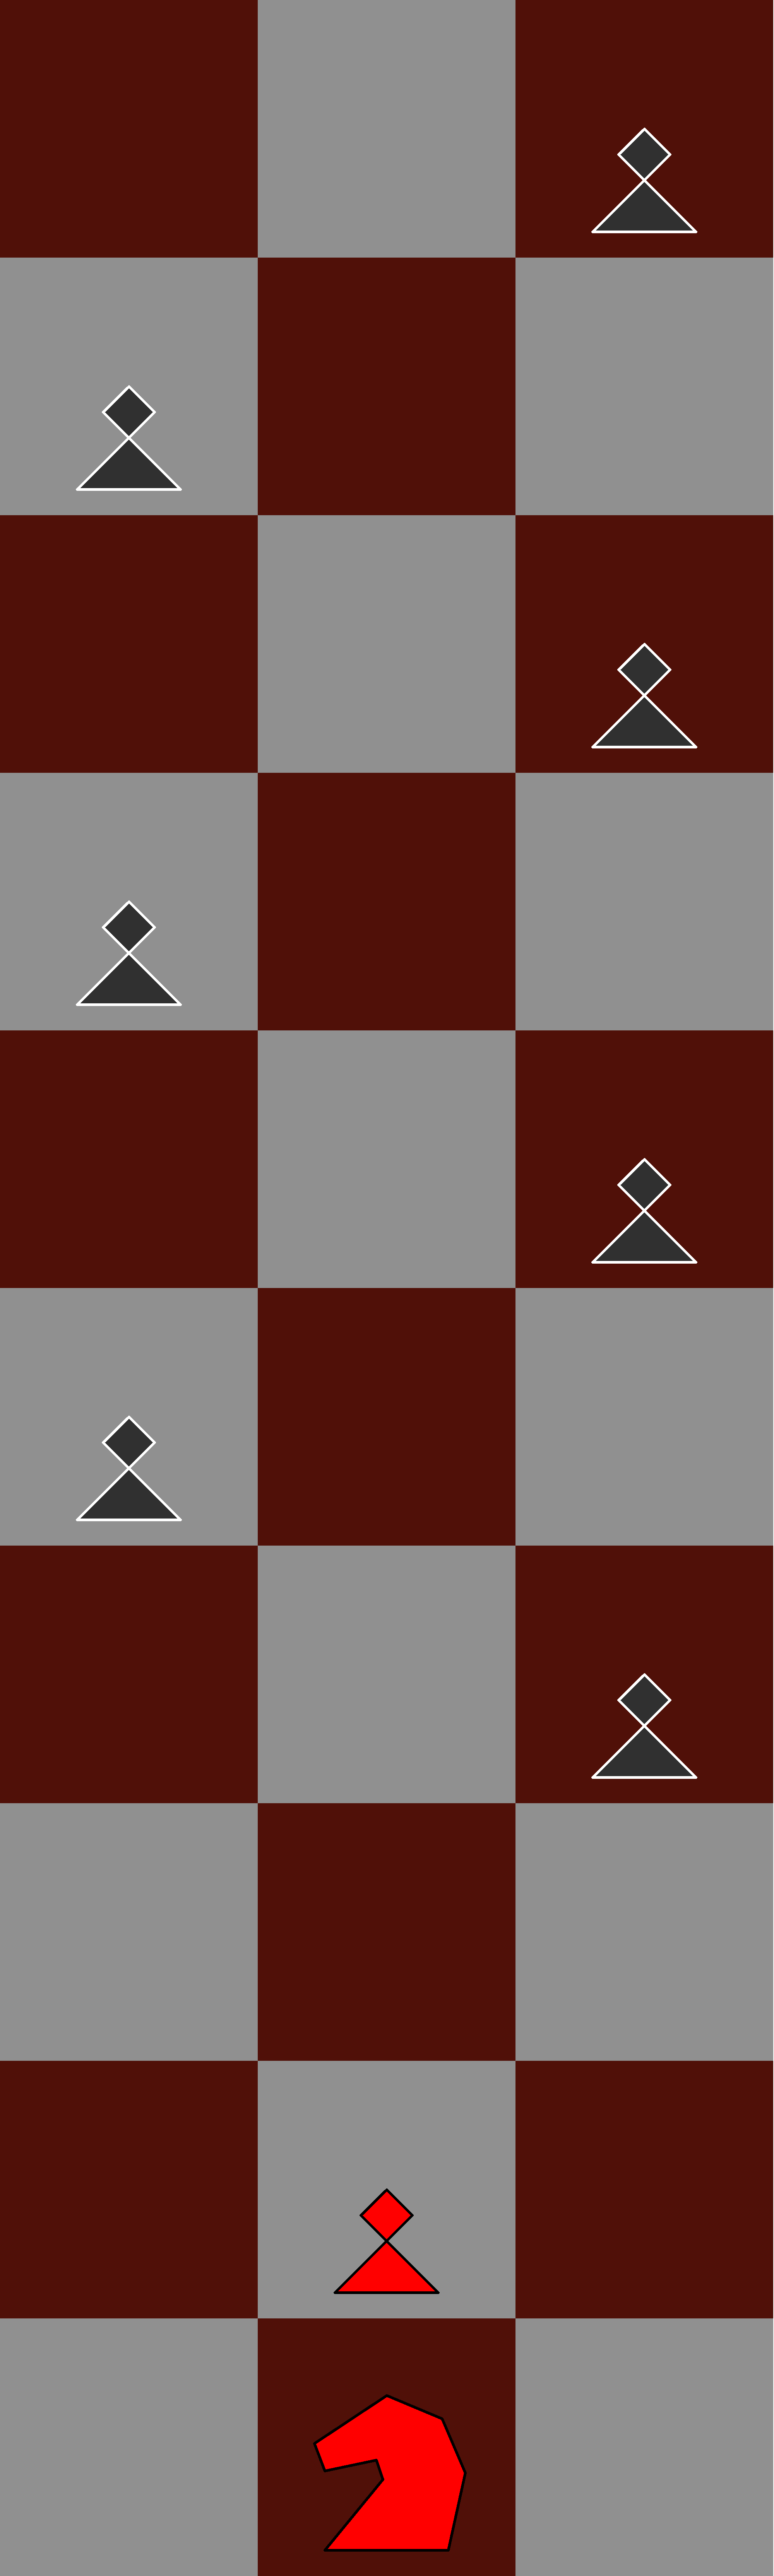
\includegraphics[width=1.0\textwidth, keepaspectratio=true]{en_passants/14_hemera_s_dawn_en_passant.png}
\caption{En passant}
\label{fig:14_hemera_s_dawn_en_passant}
\end{figure}

\TODO :: fix text, sync with Scout, Grenadier

Rush and en passant are very similar to those in
\hyperref[fig:12_nineteen_en_passant]{Nineteen variant}.
All Pawns, including scout Pawns can be rushed up to, and including, the last
row on own side of chessboard.

In this variant, Pawns can be rushed 7 (Pawn A) or 8 (B) fields, depending if
they were in first or second Pawn row. Scout Pawns can be rushed 5 (Pawn C)
or 6 (D) fields, depending how close their starting position is to opponent.

Converted opponent's Pawns cannot be rushed, even if converted on an initial
positions of own Pawns.

% \clearpage % ..........................................................

\section*{Promotion}
\addcontentsline{toc}{section}{Promotion}
\label{sec:Hemera's Dawn/Promotion}

Promotion is non enforced, delayed variety, i.e. it's the same as in
\hyperref[sec:Age of Aquarius/Promotion]{previous chess variant}, Age of Aquarius.

Promotion in this variant is polygamous, more than one Queen in the same color
can be present on chessboard at any given time.

\clearpage % ..........................................................

\section*{Castling}
\addcontentsline{toc}{section}{Castling}
\label{sec:Hemera's Dawn/Castling}

Castling is
\hyperref[sec:Nineteen/Castling]{the same as in Nineteen variant},
only difference is that King can move
between 2 and 7 fields across. All other constraints from Nineteen variant still
applies.

\noindent
\begin{figure}[!h]
\includegraphics[width=1.0\textwidth, keepaspectratio=true]{castlings/14_hd/hemera_s_dawn_castling.png}
\caption{Castling}
\label{fig:hemera_s_dawn_castling}
\end{figure}

In example above, all valid King's castling moves are numbered.

\noindent
\begin{figure}[!h]
\includegraphics[width=1.0\textwidth, keepaspectratio=true]{castlings/14_hd/hemera_s_dawn_castling_right_03.png}
\caption{Castling short right}
\label{fig:hemera_s_dawn_castling_right_03}
\end{figure}

In this example King was castling short to the right. Initial King's position is
marked with "K". After castling is finished, right Rook ends up at field immediately
left to the King.

\clearpage % ..........................................................

\section*{Initial setup}
\addcontentsline{toc}{section}{Initial setup}
\label{sec:Hemera's Dawn/Initial setup}

Compared to initial setup of Nineteen, Centaur is inserted between Bishop and Wave
symmetrically, on both sides of chessboard. This can be seen in the image below:

\noindent
\begin{figure}[h]
\includegraphics[width=1.0\textwidth, keepaspectratio=true]{boards/14_hemera_s_dawn.png}
\caption{Hemera's Dawn board}
\label{fig:14_hemera_s_dawn}
\end{figure}

\clearpage % ..........................................................
% =============================================== Hemera's Dawn chapter
